\section{Methodology}
\subsection{System Modelling}
\paragraph{}The fuel cell system model will be obtained from governing equations from which a transfer function will be generated from the linearized model. The transfer function will be used to generate a state space model for the system. 
\paragraph{}The system will then be represented in matlab and the controllers designed will be tested on the system to observe the effectiveness of each control method. 
\paragraph{} Two genral types of models are used in simulation of fuel cell technology, the approaches are detailed lumped parameter dynamic models and black-box models based on system identification. The black box model commonly expresses as NARX (Nonlinear Auto Regressive with eXogenous input) or ARMAX (Auto Regressive Moving Average with eXogenous input) equations. This project addresses both modelling approaches by presenting an ARMAX model for the black-box modelling approach and a detailed mechanistic model for the dynamic modelling approach.
\subsubsection{ARMAX Model}
\paragraph{}Hydrogen is an input variable and is fed at an adjustable flow rate N\textsubscript{H} as well as oxygen expressed as n\textsubscript{A} derived from air. Voltage and current are the system outputs. Franklin et al \cite{franklin_feedback_2002}, represent this as Multiple Input Multiple Output (MIMO) System as shown in the Figure 3.4 below.
\begin{figure}[!h]
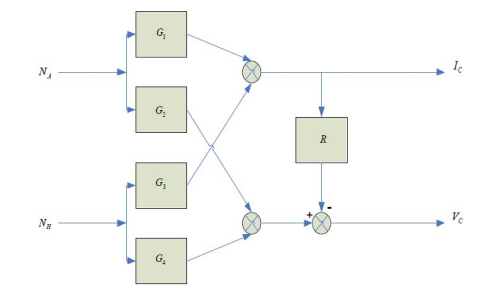
\includegraphics{Figures/mimo}
\caption{ MIMO representation of fuel cell \cite{thanapalan_model_2011}}
\end{figure}
\paragraph{}The relationship between the inputs (N\textsubscript{A} and N\textsubscript{H}) and the outputs (I\textsubscript{c} and V\textsubscript{c}), while R represents the internal resistance. The system can be represented using the following equations:
\begin{equation}
$$ V_{c} = G_{2}N_{A} + G_{4}N_{H} + RI_{C} $$
\end{equation}
\begin{equation}
$$ I_{C} = G_{1}N_{A} + G_{3}N_{H} $$
\end{equation}
\paragraph{}Equation 3.1 and 3.2 will be used as a basis for system identification and controller design.
\subsection{Simulations}
\paragraph{}From the generated models on matlab, simulations will be performed using the different controllers and the responses and other metrics will be plotted out for further analysis. Metrics such as rise time, settling time and stochastic response will be observed to determine the system performance.
\subsection{Sensors}
\paragraph{}Sensors will be used to collect data from the system as it runs. These include:
\begin{itemize}
\item Humidity sensor
\item Temperature sensor
\item Flow rate sensor
\item Pressure sensors
\item Voltage sensor
\item Current sensor
\end{itemize}
\paragraph{}These sensors will be used by the controller to observe system performance and optimize for each parameter as well as the performance requirements.
\subsection{Data Analysis}
\paragraph{}The data collected from the simulations and sensors will be analysed using custom software created using jupyter notebooks. Graphs will  be generated to compare the performance of each controller and evaluation of the selected controller.